\chapter{Introduction}
\label{chap:intro}

%%%%%%%%%%%%%%%%%%%%%%%%%%%%%%%%%%%%%%%%%%%%%%%%%%%%%%%%%%%%%%%%%%%%%%%%%%%%%%%
\section{Motivation}
\label{sec:chap1-motivation}

%Intro paragraph\\
%-talk about the increasingly important role of simulation in nuclear?\\
%-challenges for today's nuclear fleet which simulation is well-poised to tackle\\
%-segue into talk about nuclear reactor / neutron physics paragraph\\
%-important to have predictive simulation - needs to be able to extrapolate\\
%-based on empirical models\\
%-set the stage for why whole-core predictive simulation is needed!!!\\
%-need to account for angular dependence of neutron flux (e.g. "transport" methods)\\

Numerical simulation has long played an important role in nuclear reactor physics and engineering. The nuclear industry relies on computational modeling of the neutron physics in reactors to predict core reactivity, power distributions, fuel depletion, and transient behavior to ensure the safety and reliability of the current fleet of Light Water Reactors (LWRs). Predictive simulations are necessary to evaluate innovations which seek to improve reactor safety and fuel cycle economics, such as reduced safety margin uncertainties, accident-tolerant fuels, and extended cycle lengths. In addition, simulation is used to assess the technical competencies of advanced reactor technologies such as Small Modular Reactors (SMRs), Sodium Fast Reactors (SFRs), Molten Salt Reactors (MSRs), High Temperature Gas Reactors (HTGRs), among other proposed designs. 

Many Generation III+ reactors, such as the Westinghouse AP1000\texttrademark \ac{PWR}, optimize performance with complicated core designs. A variety of reactivity control mechanisms -- including partially-inserted control rods, ``grey'' control poisons, \ac{IFBA}, soluble boron, etc. -- along with axial enrichment zoning are used to improve performance metrics such as power peaking factors. The reactor analysis methods in widespread use today assume a ``smoothly'' varying flux distribution, and are not well-suited to model highly localized flux gradients which result from these complex core configurations. New high-fidelity simulation tools are needed to accurately capture neutron physics in advanced reactor designs.



next paragraph: talk about tradeoffs
-computational speed vs. accuracy, flexibility
-ability to make predictions beyond design envelope
-faster simulations enable more and faster design iterations 
-high-fi simulation used to 1) benchmark low-fi simulations and 2) inform low-fi simulations
-this thesis develops new techniques to use high fi MC to capture relevant physics in low-fi MG methods


%%%%%%%%%%%%%%%%%%%%%%%%%%%%%%%%%%%%%%%%%%%%%%%%%%%%%%%%%%%%%%%%%%%%%%%%%%%%%%%
\section{Background}
\label{sec:chap1-background}

%First paragraph\\
%-wish to replace diffusion with whole-core transport\\
%-benefits of improved reactor analysis tools\\
%-HPC may make this possible\\

The nuclear reactor physics community has long strived for whole-core transport-based tools for nuclear reactor analysis. Transport-based methods would enable more accurate core power distributions to be calculated without the approximations needed for today’s tools based upon diffusion theory. Although the computational requirements for whole-core transport-based simulations have precluded their widespread development, the continuing growth of cheap parallel processing power has made the prospects for such tools increasingly feasible.

%Second paragraph\\
%-compare contrast competing algorithms - Monte Carlo and deterministic transport\\
%-tradeoff between computational speed/efficiency and accuracy\\
%-crux of deterministic methods are MGXS\\

Core simulation tools utilizing \ac{MC} transport methods represent the ``Holy Grail'' for reactor analysis. However, the computational costs required to accommodate the slow convergence rate for \ac{MC} makes it impractical for widespread use for the foreseeable future. Deterministic transport methods pose a number of advantages to \ac{MC} from a computational perspective, which seems likely to make these methods more viable in the near to intermediate term. However, deterministic methods almost universally discretize the energy domain in a few to hundreds of energy groups. This approximation requires energy condensed \ac{MGXS} in each geometric region to preserve reaction rates. Accurate \emph{reactor agnostic} multi-group cross section generation is needed to enable deterministic transport-based methods to be as accurate and flexible as Monte Carlo in whole-core calculations.

This thesis investigates the potential use of Monte Carlo methods to generate \ac{MGXS} for next-generation whole-core deterministic reactor analyis. Monte Carlo presents a natural approach to replace engineering prescriptions to approximate the flux with a stochastic approximation of the exact flux. The advantage of a \ac{MC}-based approach is that all of the relevant physics modeled in \ac{MC} may be directly embedded into \ac{MGXS}. This improvement in accuracy comes at the computational expense of converging group constant tallies to acceptably low uncertainties. \ac{MC} methods have increasingly been used to generate few group constants for coarse mesh diffusion, most notably by the Serpent \ac{MC} code~\cite{serpent2013manual}. However, there exist few rigorous and comprehensive analyses of \ac{MGXS} generation from \ac{MGXS} for heterogeneous fine-mesh transport.

intro paragraph: whole-core transport-based methods
-look to prospectus

MC paragraph: 
-advantages in terms of ``exact'' treatment in energy, angle, space
-parallel methods (fission bank, DD, multi-threading)
-inverse square root convergence rate
-computational efficiency: poor cache efficiency, hard to vectorize
-impact of correlation on uncertainties

Deterministic paragraph: 
-non-linear convergence
-computational efficiency: structured cache efficiency, simpler to vectorize
-requires approximation to angle space and energy
-need accurate \ac{MGXS} for whole-core transport methods to be reactor agnostic

\begin{emphbox}
\textbf{The high-level vision underlying this thesis is the desire to obtain Monte Carlo-quality solutions with computationally efficient deterministic neutron transport methods.}
\end{emphbox}

next paragraph: multi-level framework
-intro MGXS
-need the flux to compute MGXS
-black magic ``crux'' of deterministic methods
-talk about decoupling of energy treatment from spatial treatment
  -successively try to embed physics effects from high-fi methods into low-fi methods
  -energy self-shielding effects first, then spatial self-shielding effects
-wish to reduce the number of stages in order to eliminate sources of approx. error and make methods more reactor agnostic or generalizable or predictive

final paragraph: MC 4 MGXS
-motivate \ac{MC} for \ac{MGXS}
-has already been done for some applications
  -esp. coarse mesh diffusion
-must accelerate it in way not possible for conventional \ac{MC}
-efforts to date still retain multi-level approach
  -new methods to consider how to eliminate the levels altogether

\begin{emphbox}
\textbf{This thesis evaluates Monte Carlo-based methods to generate \ac{MGXS} for fine mesh neutron transport codes.}
\end{emphbox}

\begin{figure}
\centering
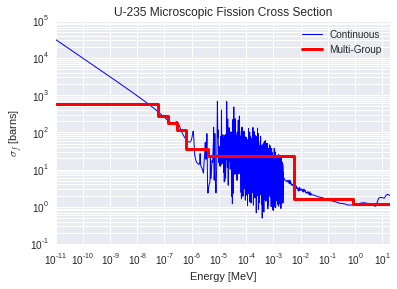
\includegraphics[width=0.9\linewidth]{figures/intro/u235-ce-mg-xs}
\caption[U-235 continuous energy and multi-group fission cross section]{U-235 continuous energy and multi-group fission cross section.}
\label{fig:chap1-multi-level-flow-chart}
\end{figure}

\begin{figure}
\centering
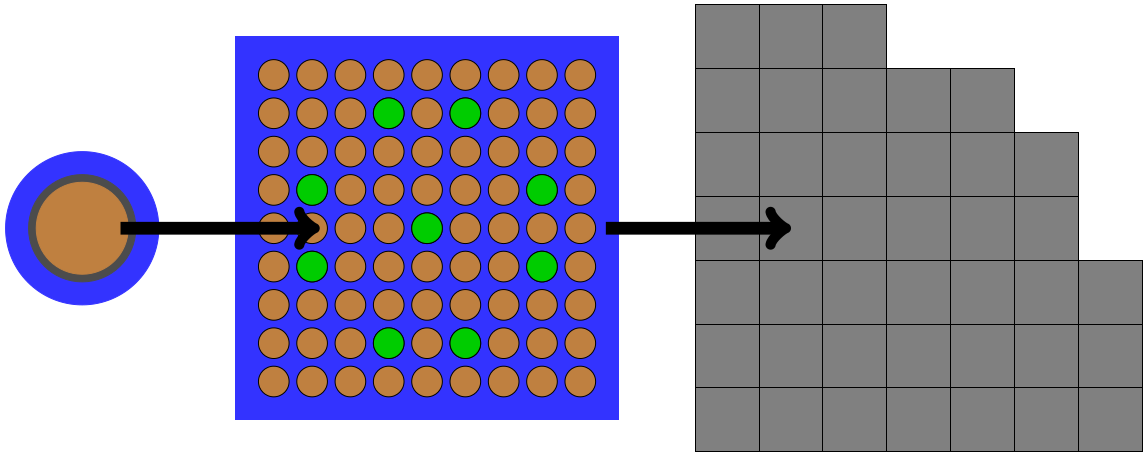
\includegraphics[width=0.9\linewidth]{figures/intro/multi-step-flow-chart}
\caption[Multi-level approach to reactor analysis]{Current multi-level framework for reactor analysis.}
\label{fig:chap1-multi-level-flow-chart}
\end{figure}


%%%%%%%%%%%%%%%%%%%%%%%%%%%%%%%%%%%%%%%%%%%%%%%%%%%%%%%%%%%%%%%%%%%%%%%%%%%%%%%
\section{Thesis Objectives}
\label{sec:chap1-objectives}

%Third paragraph\\
%-mention MG would be the reference soln anyway
%-replace deterministic approximation 
%-Existing codes/techniques may not be adequate for whole-core transport\\

-split up paragraphs according to two high-level themes
-itemize objectives with bullet points

The subject matter of this thesis can be organized along two main themes. First, the efficacy of \ac{MGXS} generation with \ac{MC} for fine-mesh transport calculations is rigorously assessed. Some of the approximations made by \ac{MC}-based \ac{MGXS} generation are quantified, including the energy- and spatial-dependence of condensed \ac{MGXS}. An in-depth analysis of systematic bias resulting from constant-in-angle \ac{MGXS} is presented, along with a scheme based on \ac{SPH} factors to compensate for this loss in accuracy. The second theme of this thesis is focused on a new methodology to simultaneously capture local and global spatial self-shielding effects in \ac{MGXS} for whole-core calcuations. This scheme applies statistical clustering to accelerate convergence rate of \ac{MGXS} tallied on high-fidelity spatial meshes in Monte Carlo. The latent variable model which inspires this new scheme is discussed. A series of increasingly complex case studies empirically compare the accuracy and convergence rate of the scheme with traditional \ac{MC}-based MGXS generation.


%%%%%%%%%%%%%%%%%%%%%%%%%%%%%%%%%%%%%%%%%%%%%%%%%%%%%%%%%%%%%%%%%%%%%%%%%%%%%%%
\section{Thesis Outline}
\label{sec:chap1-outline}

-mention that thesis is broken into three main parts
-break into two paragraphs for each part

Chapter~\ref{chap:intro} motivates the need for new \ac{MGXS} generation techniques with an overview of trends in \ac{HPC} and whole-core transport methods. Chapter~\ref{chap:mgxs} reviews the multi-group cross section approximation, and highlights past efforts to use \ac{MC} to generate \ac{MGXS}. The simulation codes utilized in this thesis are discussed in Chapter~\ref{chap:workflow}, including OpenMC, OpenMOC and OpenCG. The impact of \ac{MGXS} approxmation error is quantified in heterogeneous geometries in Chapter~\ref{chap:biases}. Chapter~\ref{chap:sph} presents an algorithmic approach to address systematic biases resulting from constant-in-angle \ac{MGXS}. A latent variable model for spatial-self shielding effects on \ac{MGXS} is outlined Chapter~\ref{chap:methods}, along with a data pipeline for unsupervised clustering to accelerate the \ac{MGXS} convergence rate. Chapter~\ref{chap:results} evaluates the impact of clustered \ac{MGXS} on the accuracy and convergence rate. Finally, Chapter~\ref{chap:conclusions} summarizes the progress made in this thesis to chart a path forward for \ac{MC}-based \ac{MGXS} generation for whole-core deterministic transport methods.

%\begin{figure}
%\begin{subfigure}{\textwidth}
%  \centering
%  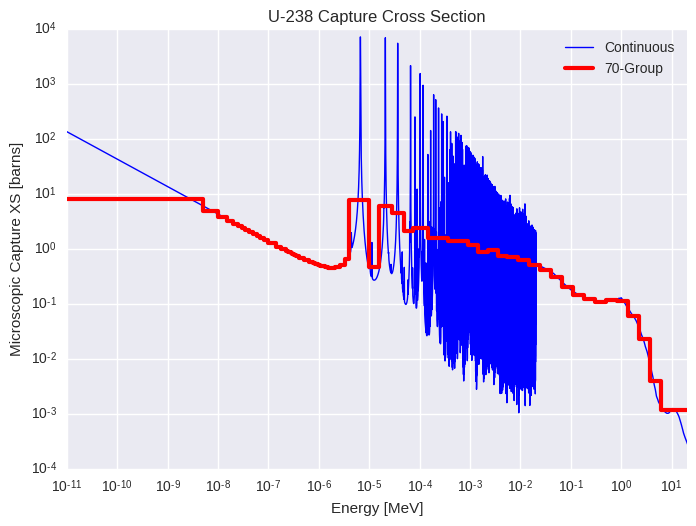
\includegraphics[width=0.9\linewidth]{figures/intro/u238-capture-70}
%  \caption{}
%\end{subfigure}
%\begin{subfigure}{\textwidth}
%  \centering
%  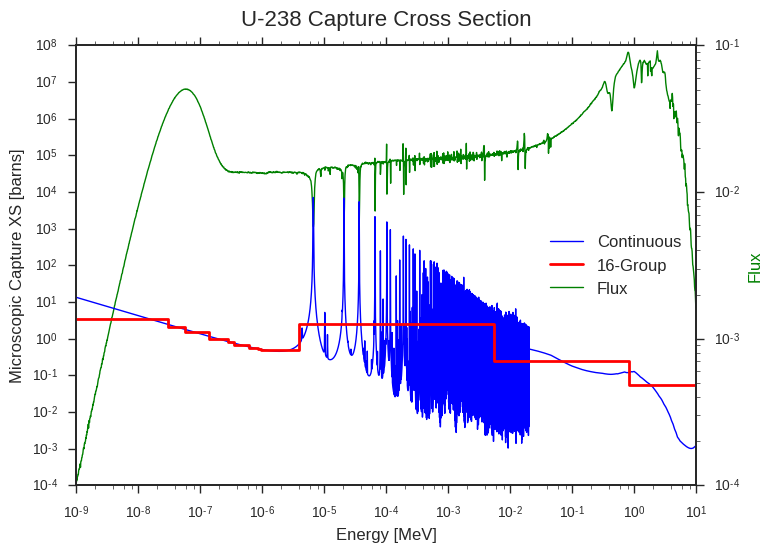
\includegraphics[width=0.9\linewidth]{figures/intro/u238-capture-16}
%  \caption{}
%\end{subfigure}
%\caption[Uranium-238 capture cross section]{Continuous energy and multi-group cross sections for U-238 capture in a PWR spectrum for 70-groups (a) and 16-groups (b).}
%\label{fig:pwr-ce-mg-xs}
%\end{figure}

